\chapter{Higher Order Fields}
\thumbforchapter{}
\chaptertoc{}
\newpage

%====================
% 	Introduction
%====================
\section{\todo{Introduction}}

Beam-based high order field measurements have been carried out in the LHC since its first
Run\todo{cite}, via chromaticity studies.
Those measurements, made by varying the RF frequency while observing the resulting tune change, have
been performed with a momentum offset of up to $\delta = \pm 2.2 \times 10^{-3}$, which led to the
observation of the third order term of the non-linear chromaticity.

During the commissioning of Run~3, a new collimator sequence has been introduced, allowing wider
momentum offset measurements, within $\delta \in [-3.2\times 10^{-3},3.7 \times 10^{-3}]$. This
improved setup led to the observation of the fourth and fifth order terms at injection energy.
Those terms, denoted $Q^{(4)}$ and $Q^{(5)}$ respectively in
\cref{eq:very_high_orders:chromaticity_high_orders}, are produced to first order by dodecapoles and
decatetrapoles. Dodecapoles being powered off at injection and decatetrapoles being absent from the
lattice, those fields originate from the field errors of the various magnets installed.

\begin{equation}
\begin{aligned}
Q(\delta) = Q_0 + Q'\delta &+ \frac{1}{2!}Q''\delta^2 + \frac{1}{3!}Q'''\delta^3
                            + \frac{1}{4!}Q^{(4)}\delta^4  + \frac{1}{5!}Q^{(5)}\delta^5
                            + \mathcal{O}(\delta^6).
\end{aligned}
    \label{eq:very_high_orders:chromaticity_high_orders}
\end{equation}

Completing measurements of high orders fields taken via chromaticity scans, turn-by-turn
measurements were also performed. High amplitude kicks indeed made the observation of dodecapolar
RDTs visible for the first time in the LHC



%=============================
%        Chromaticity
%=============================

\section{Chromaticity}


% ===============================
%         Measurement
% ===============================
\subsection{\todo{Measurement Procedure}}
\label{subsection:decapoles:chromaticity:measurement}

As described in \cref{subsection:optics_corrections_chromaticity}, the momentum offset $\delta$ is
related to the RF frequency and the momentum compaction factor. This relation is given as a
simplified form in \cref{eq:very_high_orders:simplified_eq_momentum_compaction}. 
The model $\alpha_c$ for the LHC injection optics is $3.48 \times 10^{-4}$ for beam 1 and $3.47
\times 10^{-4}$ for beam 2.  Via this relation, a change of 140Hz of the RF frequency corresponds to
a momentum offset of about $-0.001$.

\begin{equation}
    \delta = -\frac{1}{\alpha_c} \cdot \frac{\Delta f_{RF}}{f_{RF,nominal}}.
    \label{eq:very_high_orders:simplified_eq_momentum_compaction}
\end{equation}

%The standard measurement procedure is to vary the RF frequency to induce a change in momentum
%offset. Frequency steps of 20Hz are taken roughly every 30 seconds, to allow for a precise tune
%measurement. Once beam losses, registered by the beam loss monitors (BLM), are deemed too high the
%frequency is reverted back to its nominal frequency in larger steps. \cref{rf_scan} shows a typical
%RF scan performed to measure chromaticity.
%
%\begin{figure}[tbh]
%    \centering
%    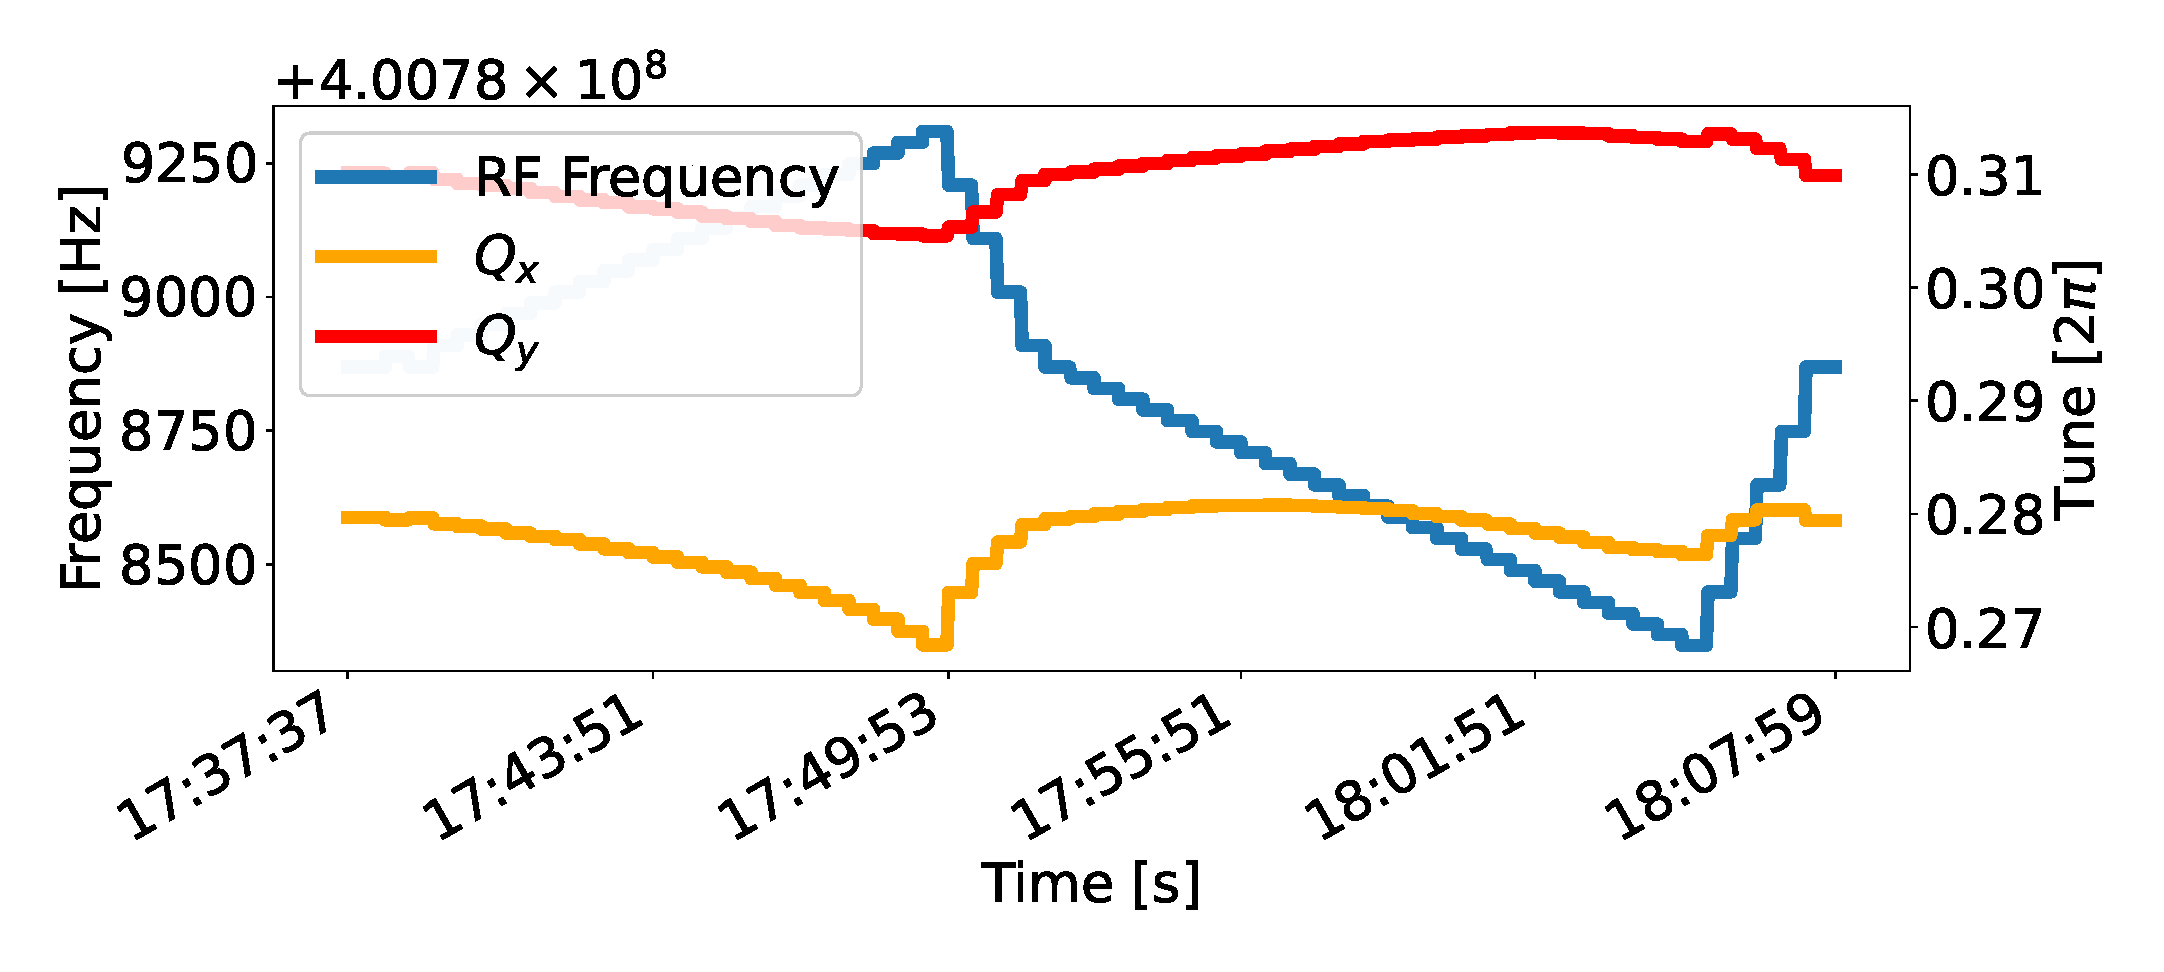
\includegraphics[width=\columnwidth]{images/MOPL027_f1-1.pdf}
%    \caption{Observation of the tune dependence on momentum offset, created by a shift of RF frequency.}
%    \label{rf_scan}
%\end{figure}

To properly characterize higher orders and ensure quality measurements, several steps are necessary.
The tune measured during chromaticity scans can exhibit jitter and resonance lines may appear,
requiring thorough data cleaning to either reject problematic data points or reduce error bars. 
The simplified \cref{eq:very_high_orders:simplified_eq_momentum_compaction}, describing $\delta$,
has been sufficient for reliably measuring up to the third order chromaticity. However, this
relation also needs verification.




% ========== Noisy Tune
\subsubsection{Noise and Spectral Lines}

Noise lines, due to electronics, can be seen in the raw data obtained from the BBQ tune system.
Occasionally, when those resonances are strong, their frequency peak can be mistaken as the tune and
logged as such by the system. This yield large uncertainties in the measurement when data points 
can't properly be classified as outliers. A tune measurement presenting this issue is showed in 
\cref{fig:decapoles:chromaticity:noisy_tune}.

\begin{figure}[H]
    \centering
    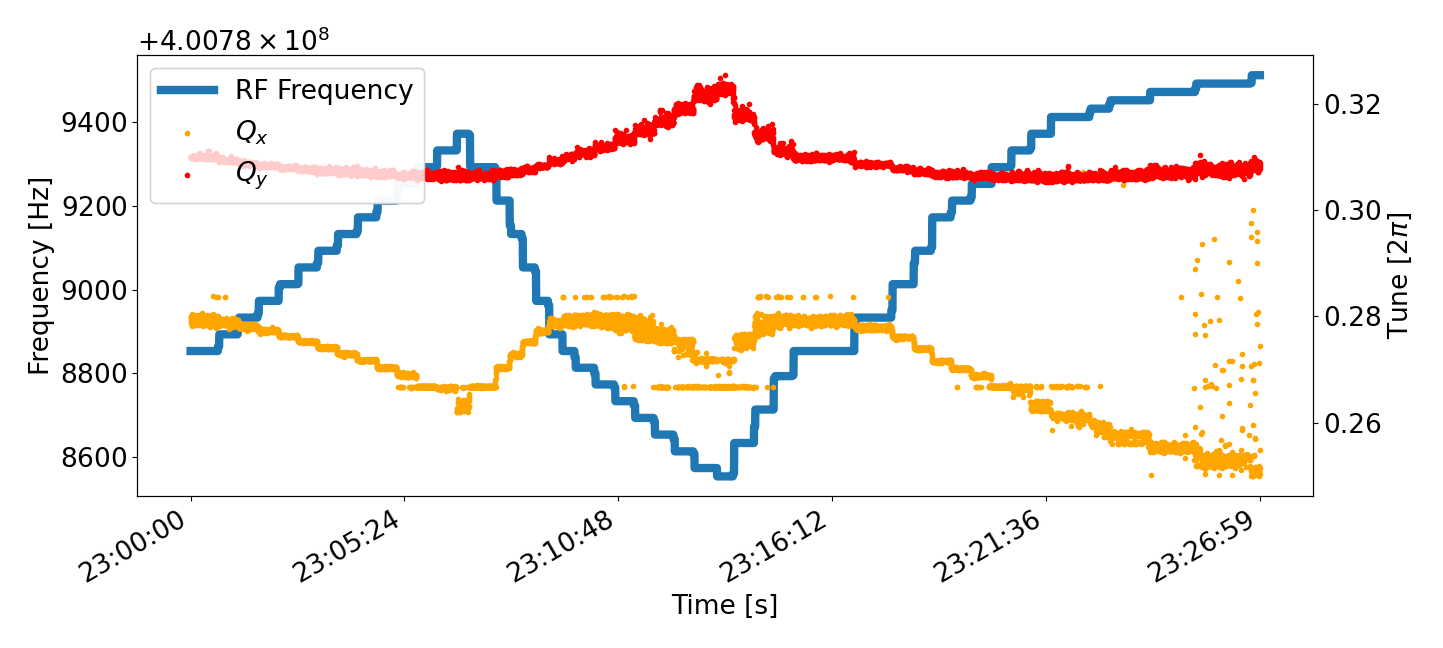
\includegraphics[width=\textwidth]{./images/noisy_tune.png}
    \caption{Shift of the tune by variation of the RF. Noise lines can appear in some cases,
    making the tune error bar large or downright unusable.}
    \label{fig:decapoles:chromaticity:noisy_tune}
\end{figure}

A solution to this issue is to use the raw data extracted from the BBQ system. From there, a
spectrogram clearly shows the noise lines, as seen in \cref{fig:decapoles:chromaticity:spectrogram}.
Those lines have been repeatedly identified over several measurements and confirmed to be fixed.
The highest peak of the spectrogram can thus be safely identified by removing those resonances,
yielding a cleaner measurement. It is also to be added that the BBQ requires to set a tune window,
which can be forgotten. By analyzing the raw data, it is ensured that the measurement has usable
data and does not try to measure noise.

\begin{figure}[H]
    \centering
    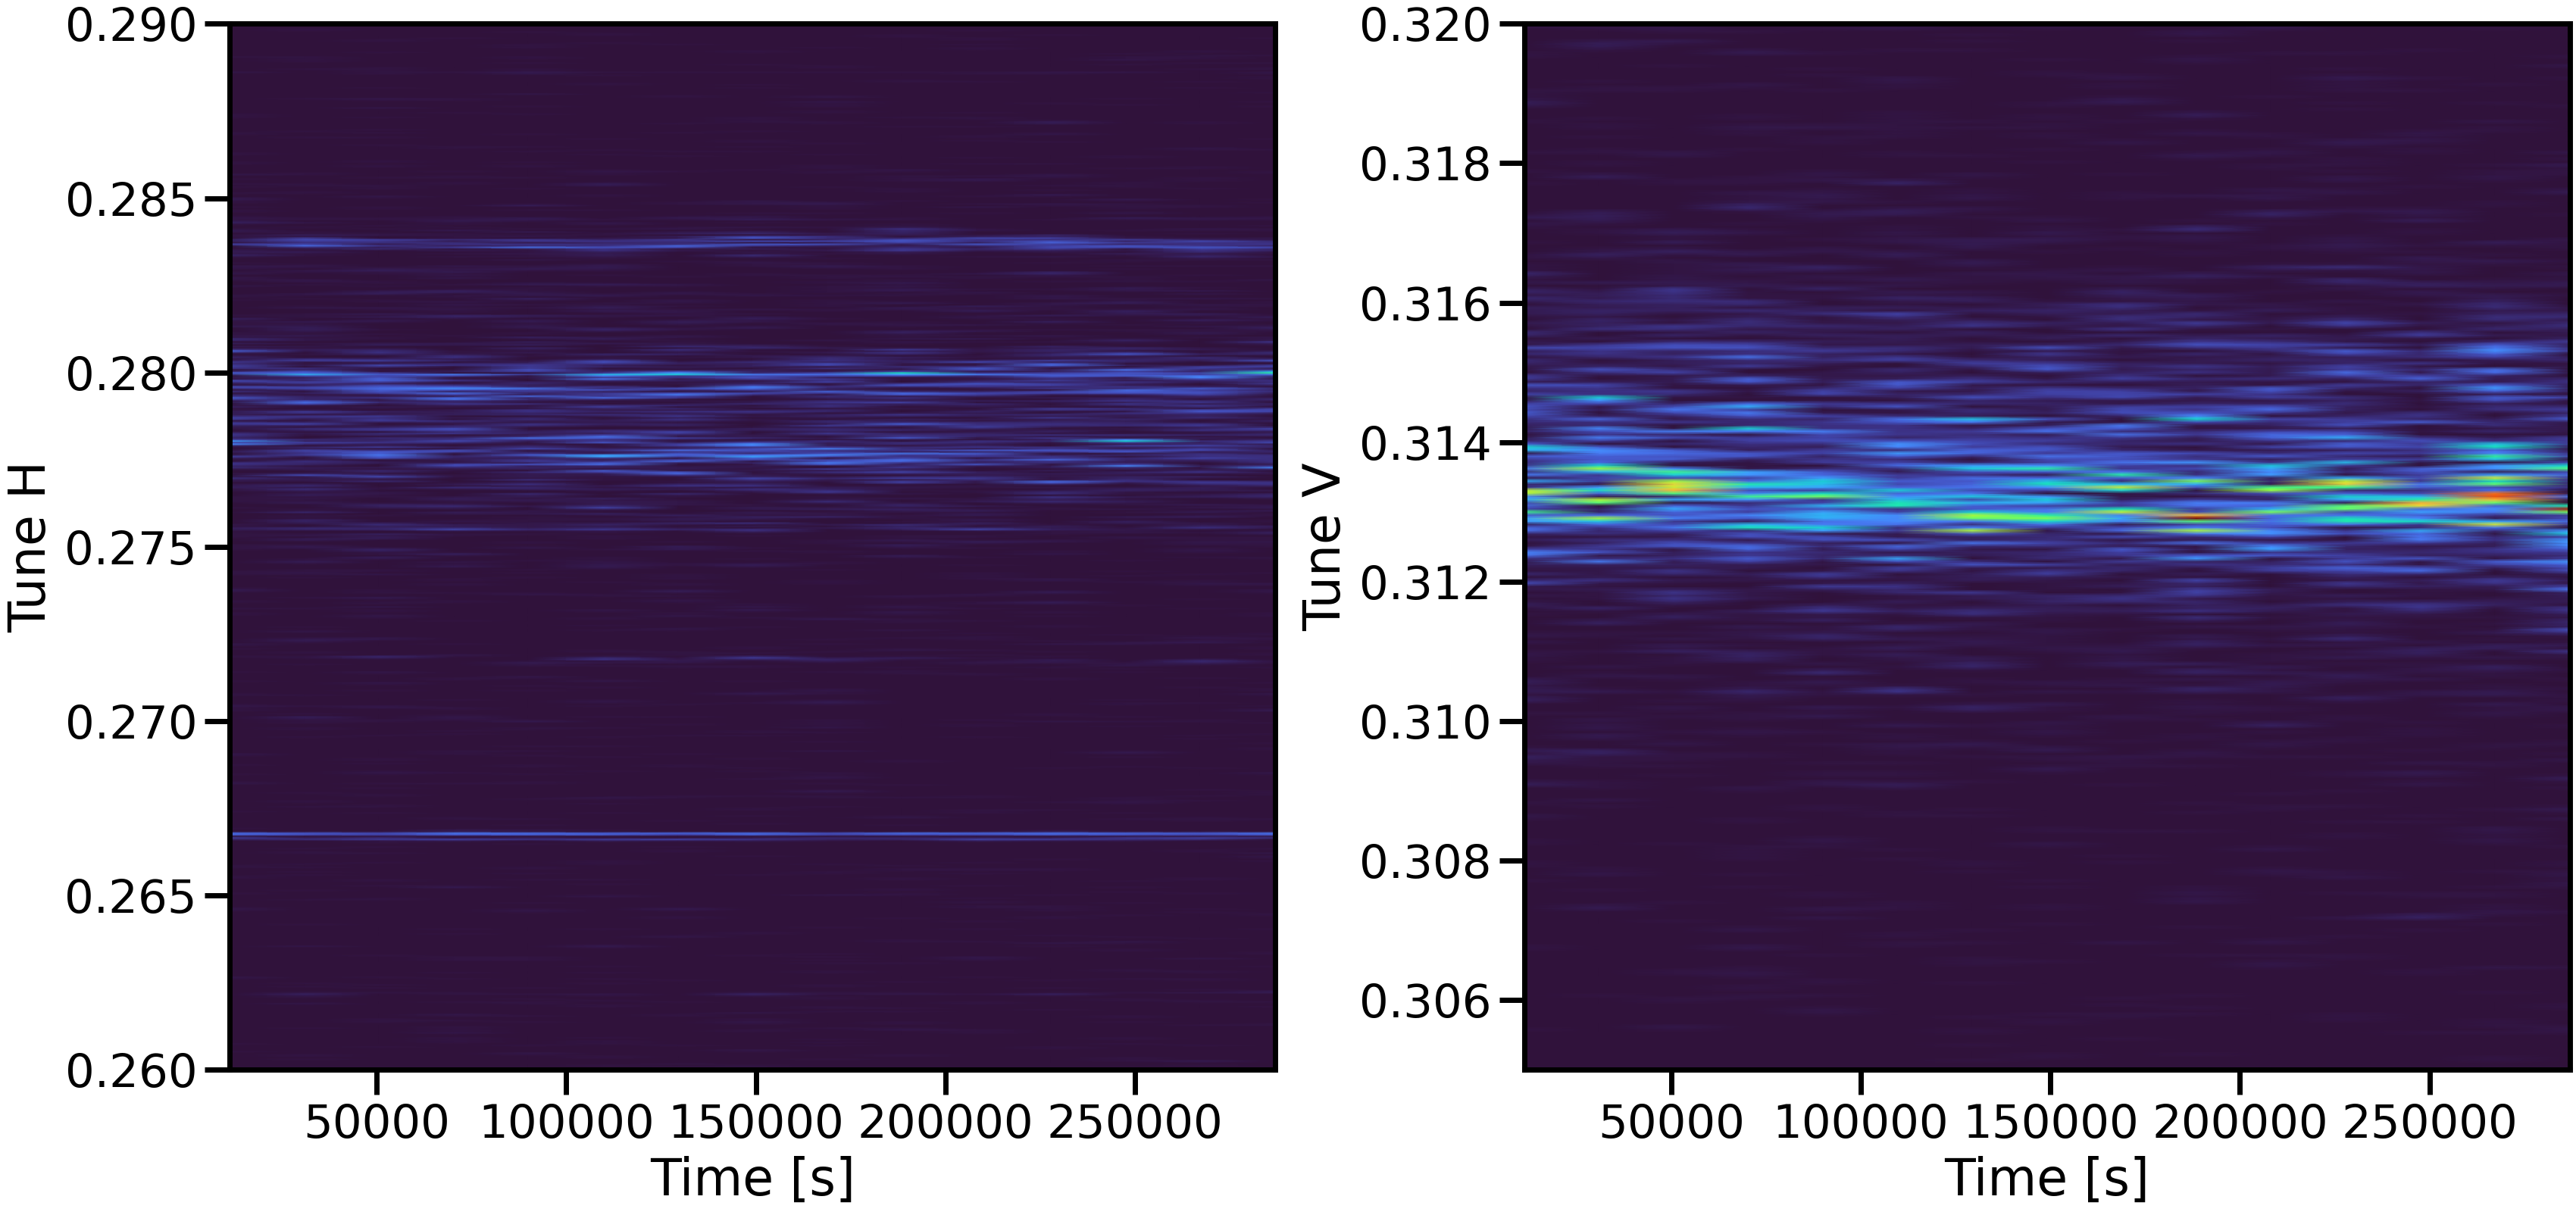
\includegraphics[width=.8\textwidth]{./images/spectrogram.png}
    \caption{Tune spectrogram obtained via BBQ system. Strong resonance lines can be seen above and
    below where the tune really is, causing the wrong frequency peak to be identified as the tune.}
    \label{fig:decapoles:chromaticity:spectrogram}
\end{figure}



% ========== Momentum Compaction Factor
\subsubsection{\review{Momentum Compaction Factor}}
\label{subsubsection:momentum_compaction_factor_studies}

Rather than a constant, the momentum compaction factor can be expressed as an
expansion, as detailed in~\cref{subsection:coordinates_systems:momentum_compaction_factor}.
The first terms are given by the following,

\begin{equation}
    \alpha_c = 
    \underbrace{\alpha_{c,0}}_{1^\text{st} \text{ order}}
    + \underbrace{\alpha_{c,1} \delta}_{2^\text{nd} \text{ order}}
    + \underbrace{\alpha_{c,2} \delta^2}_{3^\text{rd} \text{ order}}.
\end{equation}

The expression for $\delta$ at first and second order then reads,

\begin{equation}
    \begin{aligned}
        \delta &= -\frac{\Delta f_{RF}}{\alpha_{0} f_{RF}} && \Rightarrow \text{Order 1} \\
        \delta &= \frac{- \alpha_{0} f_{RF} + \sqrt{f_{RF} 
            \left(- 4 \Delta f_{RF} \alpha_{1} + \alpha_{0}^{2} f_{RF}\right)}}{2 \alpha_{1} f_{RF}}
            && \Rightarrow \text{Order 2} 
    \end{aligned}
\end{equation}

It is assumed that only the first term is relevant as the induced difference in chromaticity is
negligible as will be demonstrated later on.
\cref{fig:decapoles:chromaticity:momentum_compaction_factor} shows the non linearity of the momentum
compaction factor and its effect on the calculated $\delta$ via the previous formulas.

\begin{figure}[tbh]
    \centering
    \begin{subfigure}[t]{0.48\textwidth}
        \centering
        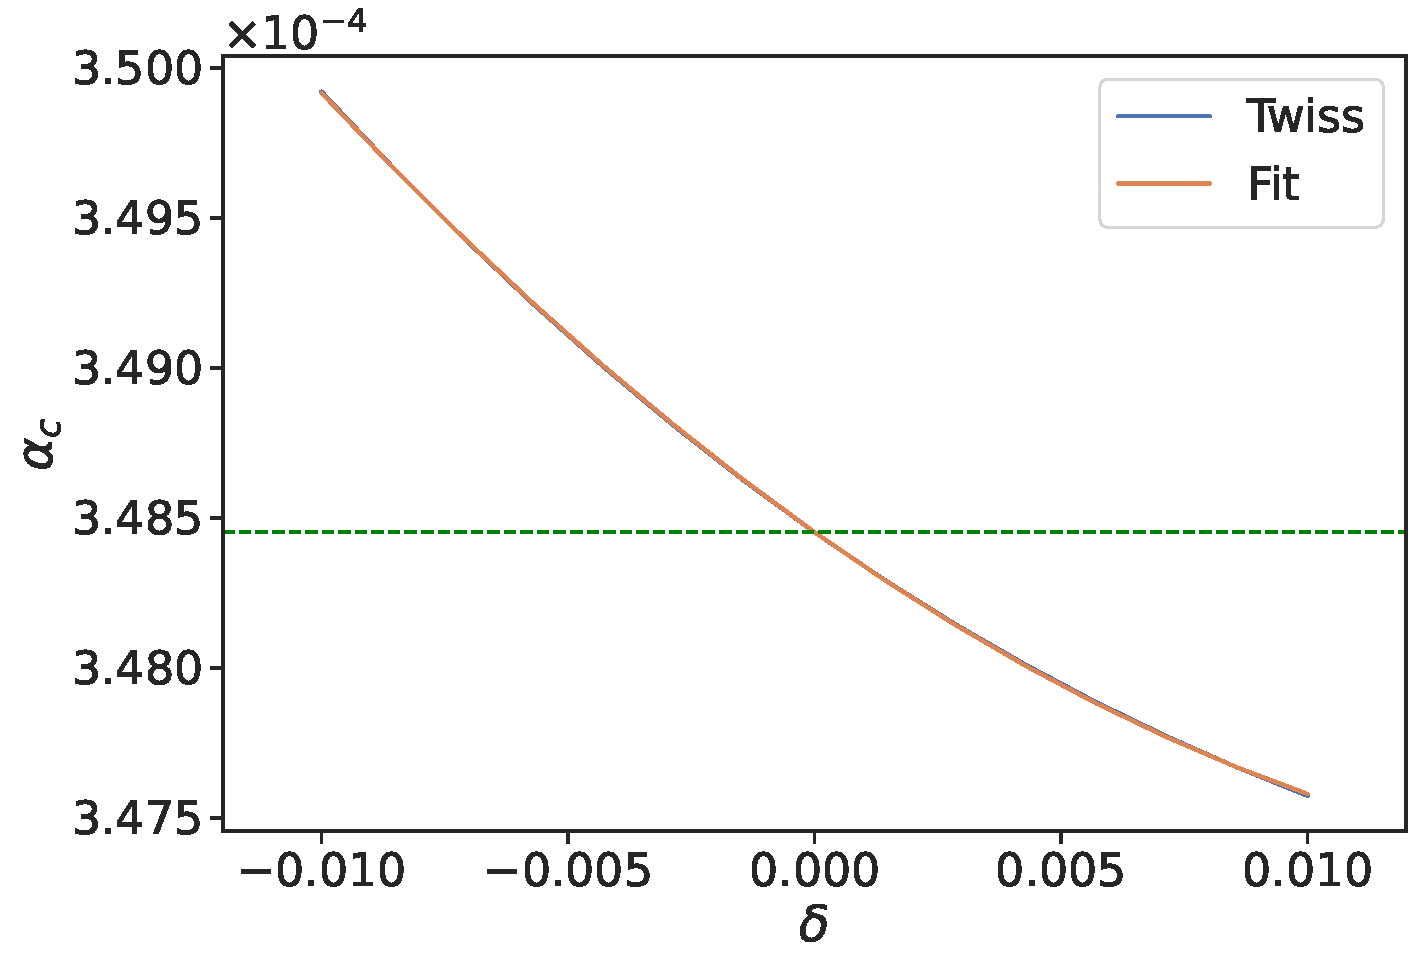
\includegraphics[width=\textwidth]{images/higher_order_momentum_compaction_factor.pdf}
        \caption{Non-linear fit of $\alpha_c$ obtained via an evaluation at discrete $\delta$ in
        MAD-X. The green line represents a constant $\alpha_c = \alpha_{c,0}$.}
    \end{subfigure}
    \hfill
    \begin{subfigure}[t]{0.48\textwidth}
        \centering
        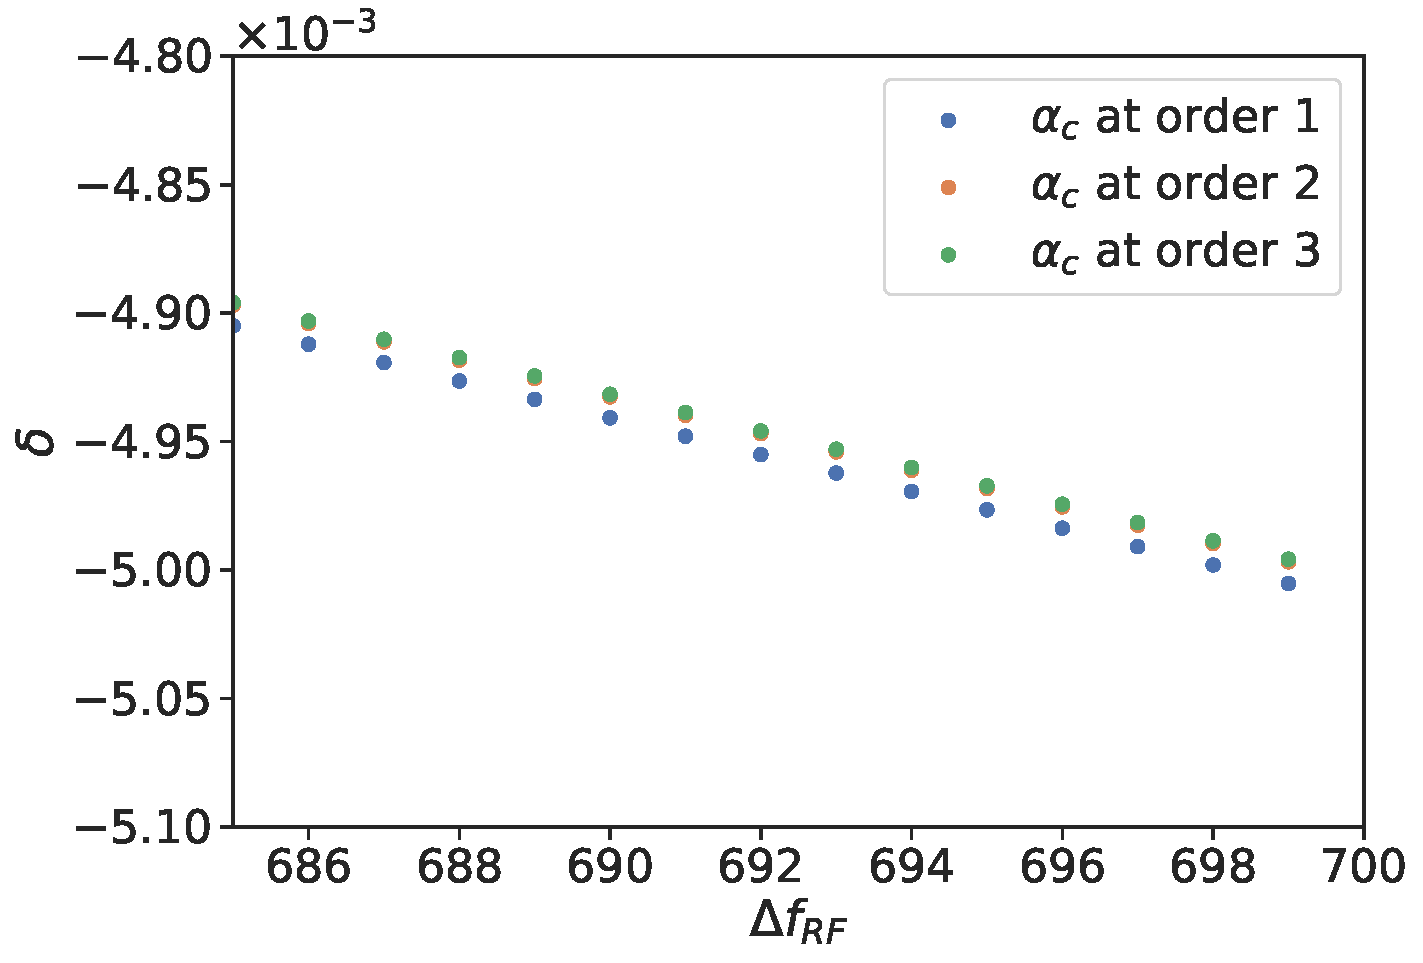
\includegraphics[width=\textwidth]{images/delta_vs_frf_alpha_c.pdf}
        \caption{Divergence of the momentum offset when considering higher $\alpha_c$ orders with
        large RF trims.}
    \end{subfigure}
    \caption{Non linearity of $\alpha_c$ and its effect on the computed $\delta$ via RF trims. The
    simulations are done at injection energy of 450GeV.}
    \label{fig:decapoles:chromaticity:momentum_compaction_factor}
\end{figure}

It is observed that while clearly depending on higher orders, the momentum compaction factor only
has a small impact on the calculated $\delta$.
\cref{fig:decapoles:chromaticity:momentum_compaction_factor_chroma_meas} shows a real-life 
measurement, comparing the fit of the chromaticity function with various $\delta$, computed up to
the third order of $\alpha_c$.

\begin{figure}[tbh]
    \centering
    \begin{subfigure}[t]{0.48\textwidth}
        \centering
        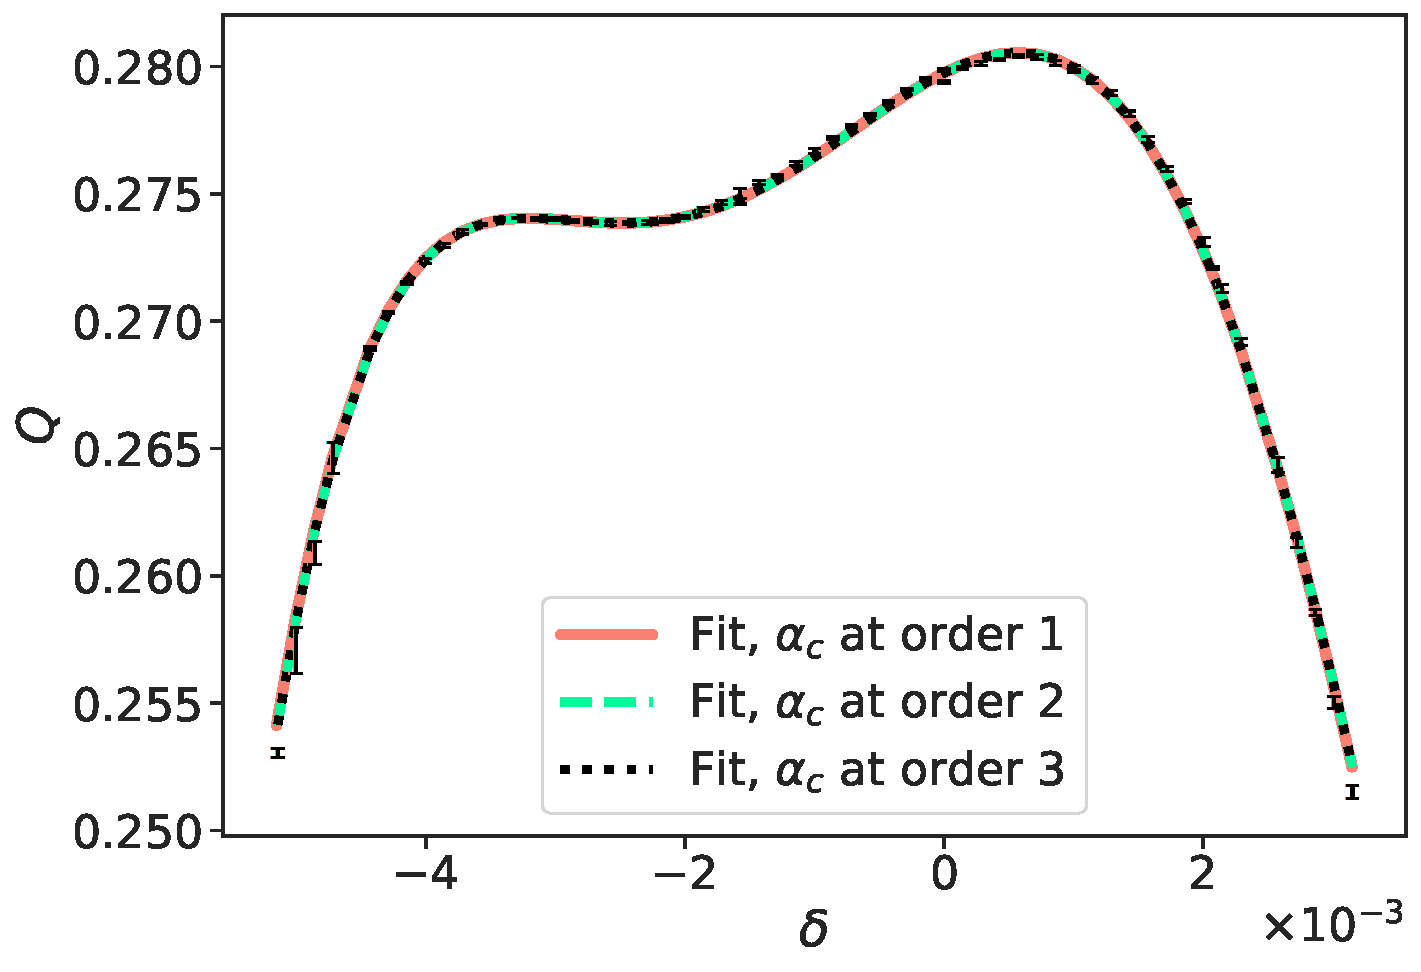
\includegraphics[width=\textwidth]{images/chroma_function_alpha_c.pdf}
        \caption{Fit of the chromaticity function at the $5^{\text{th}}$ order, considering the
        $\alpha_c$ expansion up to the third order.}
    \end{subfigure}
    \hfill
    \begin{subfigure}[t]{0.48\textwidth}
        \centering
        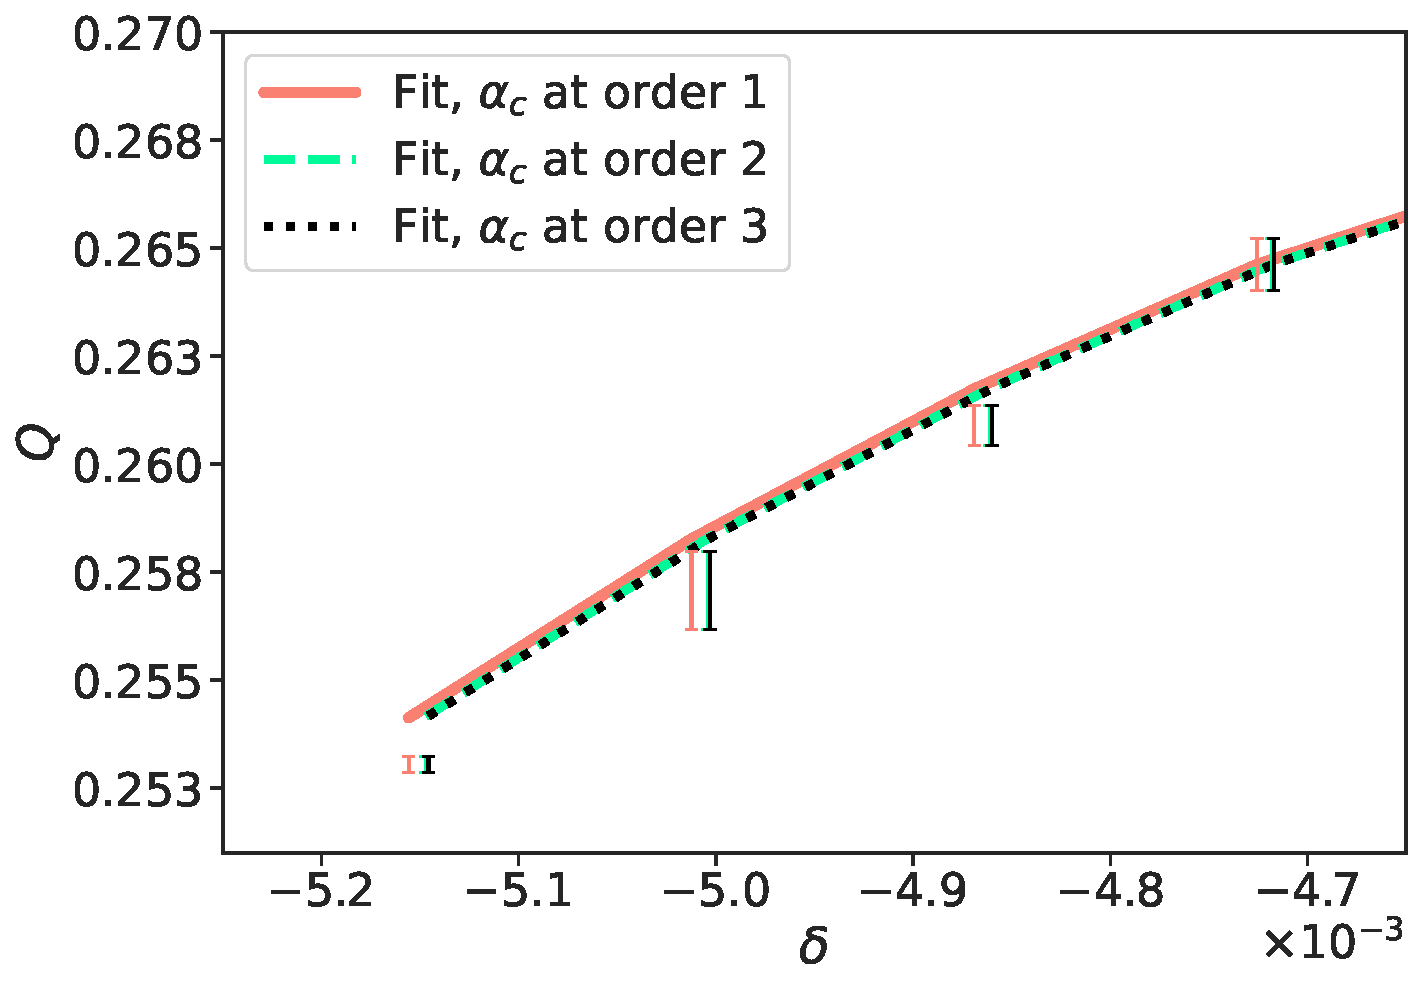
\includegraphics[width=\textwidth]{images/chroma_function_alpha_c_zoom.pdf}
        \caption{Zoom on one side of the fit. The difference between the second and third order
        is barely noticeable.}
    \end{subfigure}
    \caption{Fit of the chromaticity function considering several $\alpha_c$ orders.}
    \label{fig:decapoles:chromaticity:momentum_compaction_factor_chroma_meas}
\end{figure}

The fit of the chromaticity function is barely impacted when considering the higher orders of the 
momentum compaction factor. The different orders of the chromaticity are collected
in~\cref{table:decapoles:chromaticity:alpha_c_chroma}.
The higher order terms of $\alpha_c$ can thus be neglected and are not a source of higher
chromaticity orders.

\begin{table}[tbh]
    \begin{tabular}{c|ccccc}
        $\alpha_c$ Order & $Q^{(1)}$ & $Q^{(2)}$ & $Q^{(3)}$ & $Q^{(4)}$ & $Q^{(5)}$\\
        \hline
        1 & 2.52 ± 0.03 & -3.04 ± 0.05 & -4.75 ± 0.03 & -0.33 ± 0.07 & 2.33 ± 0.06 \\
        2 & 2.53 ± 0.03 & -3.05 ± 0.05 & -4.75 ± 0.03 & -0.32 ± 0.07 & 2.36 ± 0.06 \\
        3 & 2.53 ± 0.03 & -3.05 ± 0.05 & -4.75 ± 0.03 & -0.32 ± 0.07 & 2.36 ± 0.06 \\
        \end{tabular}
    \caption{}
    \label{table:decapoles:chromaticity:alpha_c_chroma}
\end{table}



%----------------------------------------
%         Other dpp Measurements
%----------------------------------------
\subsubsection{Momentum Offset from Orbit}

During machine operation, the momentum offset, derived from the orbit, used to be logged on the
servers. It was then possible to directly compute the chromaticity that way without having to use
the RF and the momentum compaction factor.
In 2016, measurements of the non-linear chromaticity were performed using the former method.
\cref{fig:very_high_orders:bare_chroma_2016} shows a comparison of the obtained non-linear 
chromaticity from both methods, while \cref{table:very_high_orders:bare_chroma_2016} shows a
numerical comparison. Results being similar, is it deemed that both methods are reliable to measure
the non-linear chromaticity in the LHC.

\begin{figure}[H]
    \begin{subfigure}{0.49\textwidth}
        \centering
        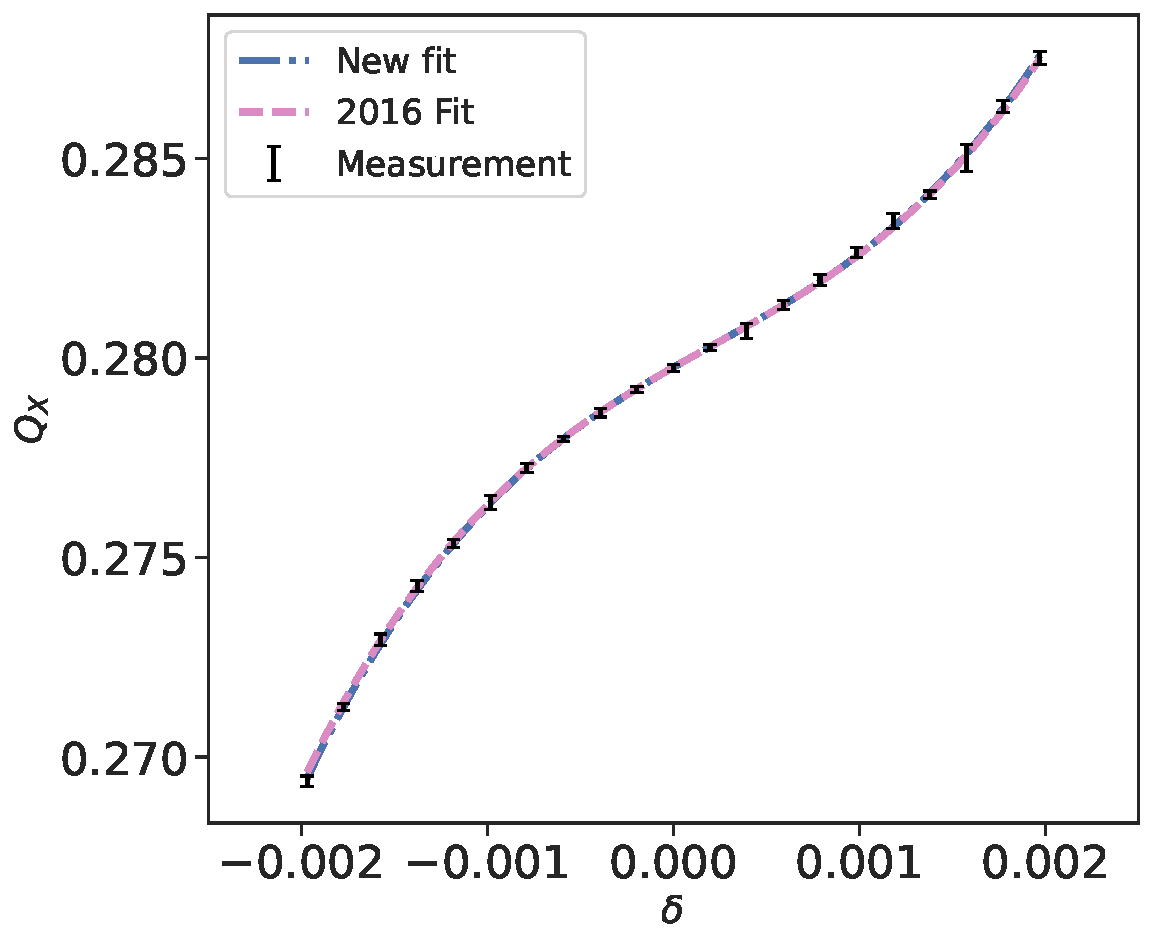
\includegraphics[width=\textwidth]{./images/chromaticity_2016/B1_qx.pdf}
        \caption{$Q_x$ Beam 1}
        \label{}
    \end{subfigure}
    \hfill
    \begin{subfigure}{0.49\textwidth}
        \centering
        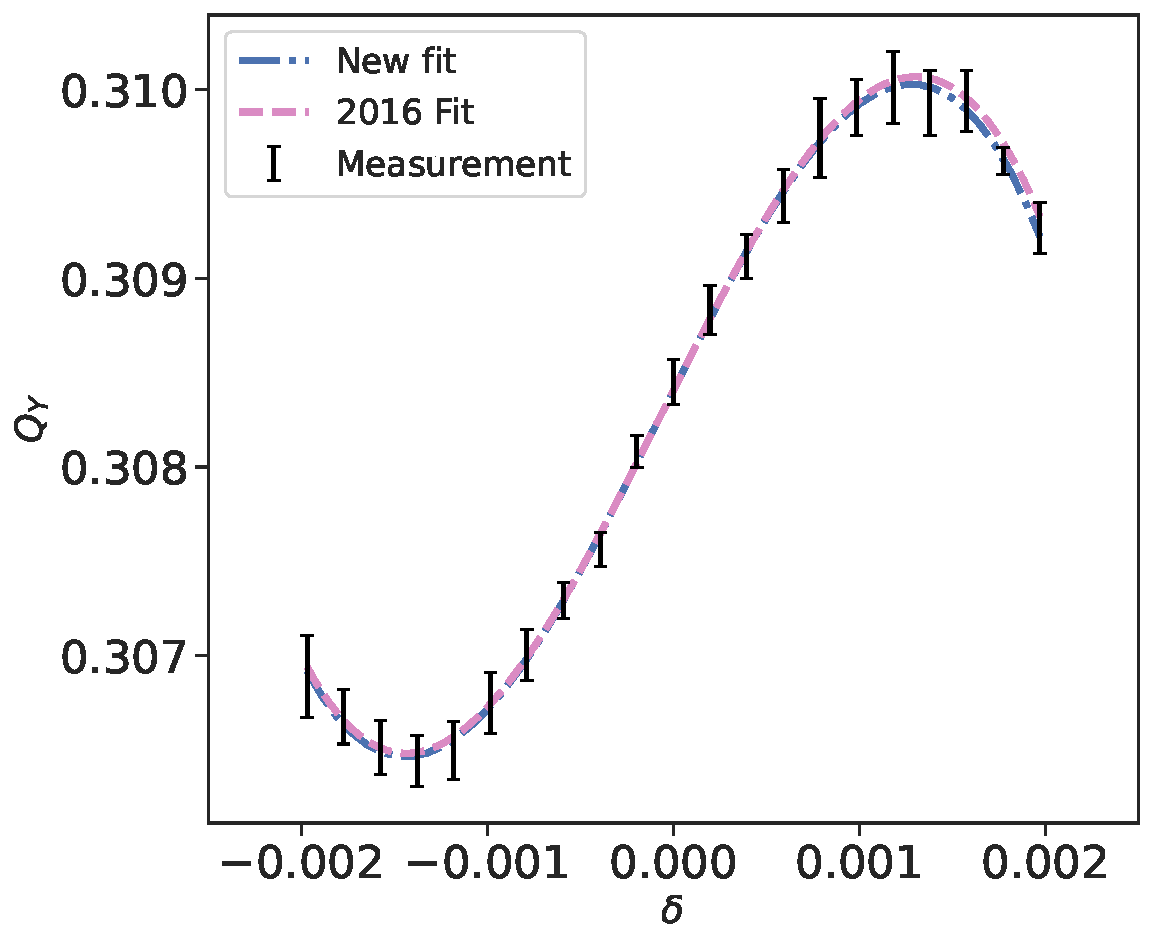
\includegraphics[width=\textwidth]{./images/chromaticity_2016/B1_qy.pdf}
        \caption{$Q_y$ Beam 1}
        \label{}
    \end{subfigure}
    %
    \\
    %
    \begin{subfigure}{0.49\textwidth}
        \centering
        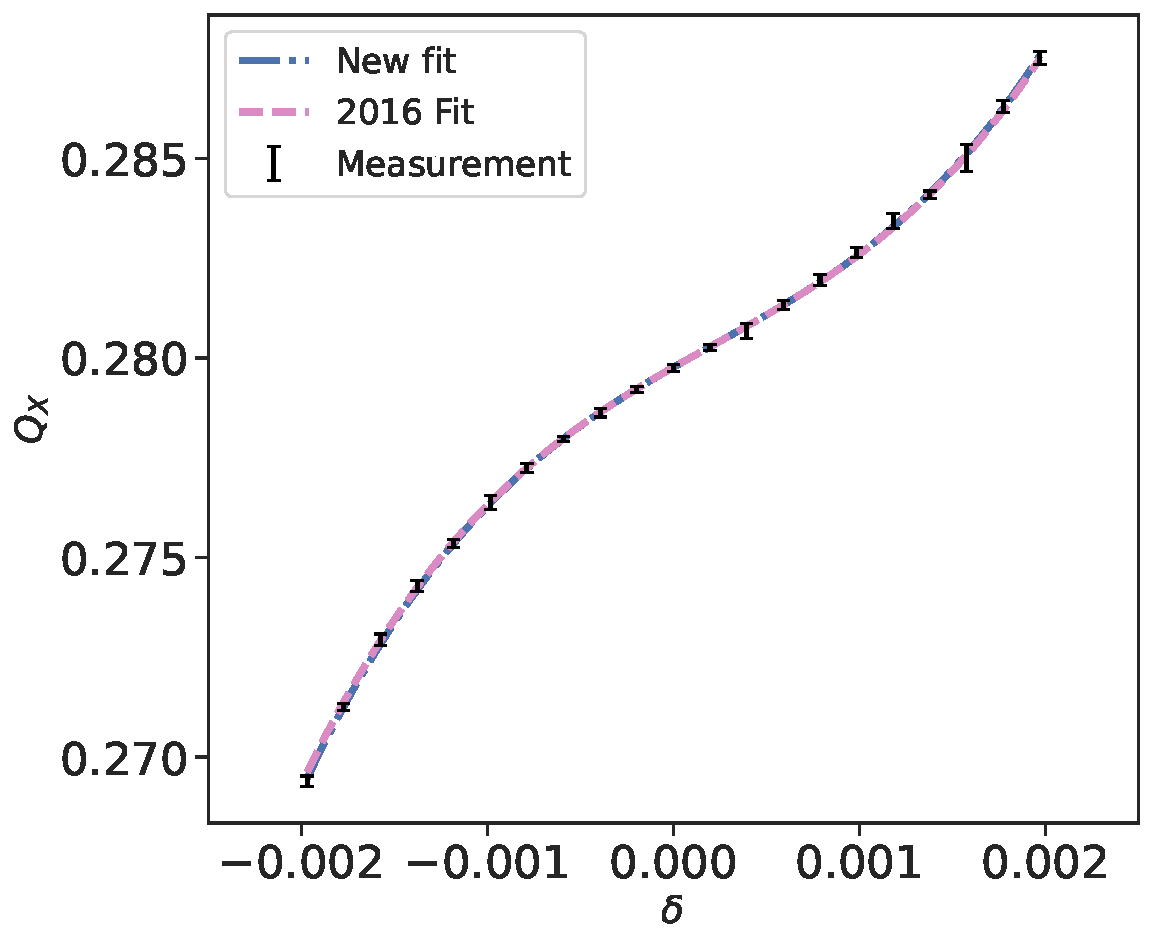
\includegraphics[width=\textwidth]{./images/chromaticity_2016/B1_qx.pdf}
        \caption{$Q_x$ Beam 2}
        \label{}
    \end{subfigure}
    \hfill
    \begin{subfigure}{0.49\textwidth}
        \centering
        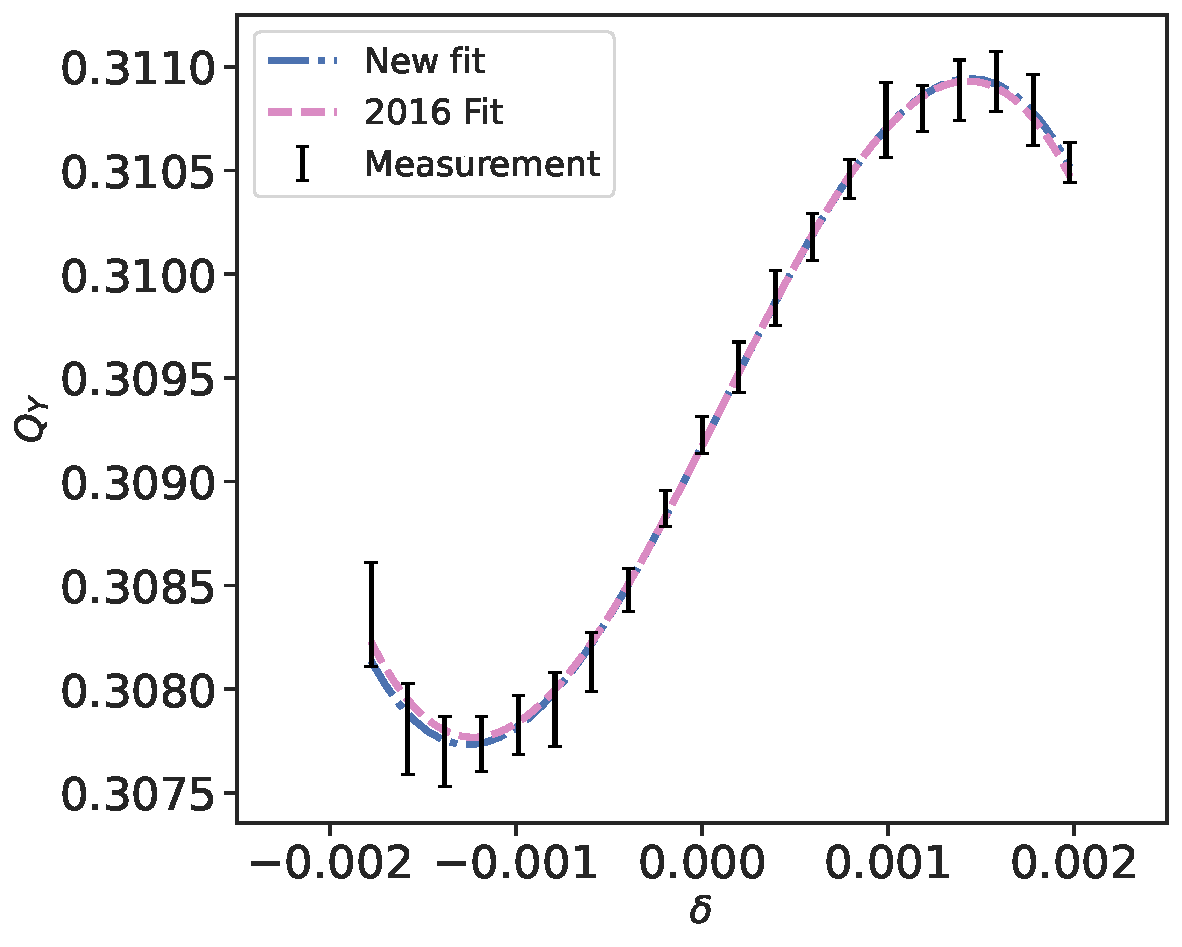
\includegraphics[width=\textwidth]{./images/chromaticity_2016/B2_qy.pdf}
        \caption{$Q_y$ Beam 2}
        \label{}
    \end{subfigure}
    \caption{Comparison of the non-linear chromaticity fit obtained from the computed momentum
    offset via the RF in 2022 and from the logged values in 2016.}
    \label{fig:very_high_orders:bare_chroma_2016}
\end{figure}

\begin{table}[H]
    \centering
    \begin{tabular}{|l||rr|rr|}
        \hline
        \multicolumn{1}{|c||}{} & \multicolumn{2}{c|}{2022}       &  \multicolumn{2}{c|}{2016} \\
            & $Q'' [x10^3]$ & $Q''' [x10^6]$ & $Q'' [x10^3]$ & $Q''' [x10^6]$\\
        \hline \hline
        B1 &&&& \\
        X & -0.64 ± 0.01 &   3.0 ± 0.04   & -0.62 ± 0.01 &  2.91 ± 0.04 \\
        Y & -0.17 ± 0.01 & -2.12 ± 0.04   & -0.14 ± 0.01 & -2.09 ± 0.04 \\
        \hline
        B2 &&&& \\
        X & -1.18 ± 0.02 &  2.89 ± 0.06   & -1.23 ± 0.03 &  3.13 ± 0.11 \\
        Y &  0.18 ± 0.02 & -1.95 ± 0.05   &  0.20 ± 0.02 & -2.02 ± 0.06 \\
        \hline
    \end{tabular}
    \label{table:very_high_orders:bare_chroma_2016}
    \caption{\todo{blablabla!}}
\end{table}



%----------------------------------------
%        Performed Measurements
%----------------------------------------
\subsection{Performed Measurements}

In order to assess the correctness of the observation of higher chromaticity orders, measurement
repeatability is needed. Two measurements were thus taken, with different configurations pertaining
top the correction of the second and third order chromaticities $Q''$ and $Q'''$.

Those two chromaticity measurements were indeed performed with different settings. The first one
used the nominal correction strengths for octupole and decapole corrector magnets, derived from
magnetic measurements, where the second one used beam-based corrections for the same elements,
computed from measurements. 
Those two measurements have a respective momentum-offset range of $[-3.1 \times 10^{-3}, 3.1 \times
10^{-3}]$ and $[-3.2 \times 10^{-3}, 3.7 \times 10^{-3}]$.

In order to stay consistent, both measurements saw their horizontal and vertical tunes respectively
set to $Q_x = 0.28$ and $Q_y = 0.31$. The linear chromaticity $Q'$ is set to a small value of $2$ to
avoid large tune shifts.


%----------------------------------------
%          Nominal Corrections
\subsubsection{Nominal Corrections}

This first chromaticity measurement was performed during the LHC beam commissioning in April 2022,
as part of the routine measurements and corrections performed after every technical of long
shutdown.
The octupole and decapole correctors were set to their nominal settings, aimed at correcting $Q''$
and $Q'''$, as previously described in \todo{ref decapole chapter}.

Results of this initial measurement are shown in Tab. \ref{chroma_fidel}. Lower order chromaticities such as
$Q'$ and $Q''$ are consistent with previous measurements~\cite{maclean_commissioning_2016}.

\begin{table}[tbh]
    \centering
    \small
    \setlength{\tabcolsep}{4.2pt}
    \begin{tabular}{|l||r|r|r|r|}
    \hline
                  & $Q^{(2)} [10^3]$ & $Q^{(3)} [10^6]$ & $Q^{(4)} [10^9]$ & $Q^{(5)} [10^{12}]$ \\ \hline\hline
        B1        &              &               &              & \\
        X         & -2.44 ± 0.02 & -3.36 ± 0.04 & -0.56 ± 0.02  &  1.20 ± 0.07 \\
        Y         &  0.97 ± 0.02 &  1.62 ± 0.05  &  0.15 ± 0.03 & -0.88 ± 0.09 \\ \hline
        B2        &              &               &              & \\
        X         & -2.45 ± 0.03 & -2.72 ± 0.08 & -1.00 ± 0.05  &  0.15 ± 0.14 \\
        Y         &  0.79 ± 0.03 & 1.54 ± 0.06  &  0.24 ± 0.04  & -0.74 ± 0.13 \\ \hline
    \end{tabular}
    \caption{Terms of the high order chromaticity obtained during Run~3 commissioning in April 2022, with nominal corrections.}
    \label{chroma_fidel}
\end{table}

Due to the momentum offset being zero several times during the measurement, it was possible to determine that
the tune drift is negligible. The measurement was also performed after an extended period at injection
energy, where the $b_3$ decay is small and not causing any change in the first order chromaticity.
The fitted curve for the chromaticity function is shown in Fig. \ref{chroma_before_correction}.
It can be seen that a higher order polynomial is beneficial for the fit, as discussed further in~"\nameref{subsection:q4q5_quality}".


\begin{figure}[tbh]
    \centering
    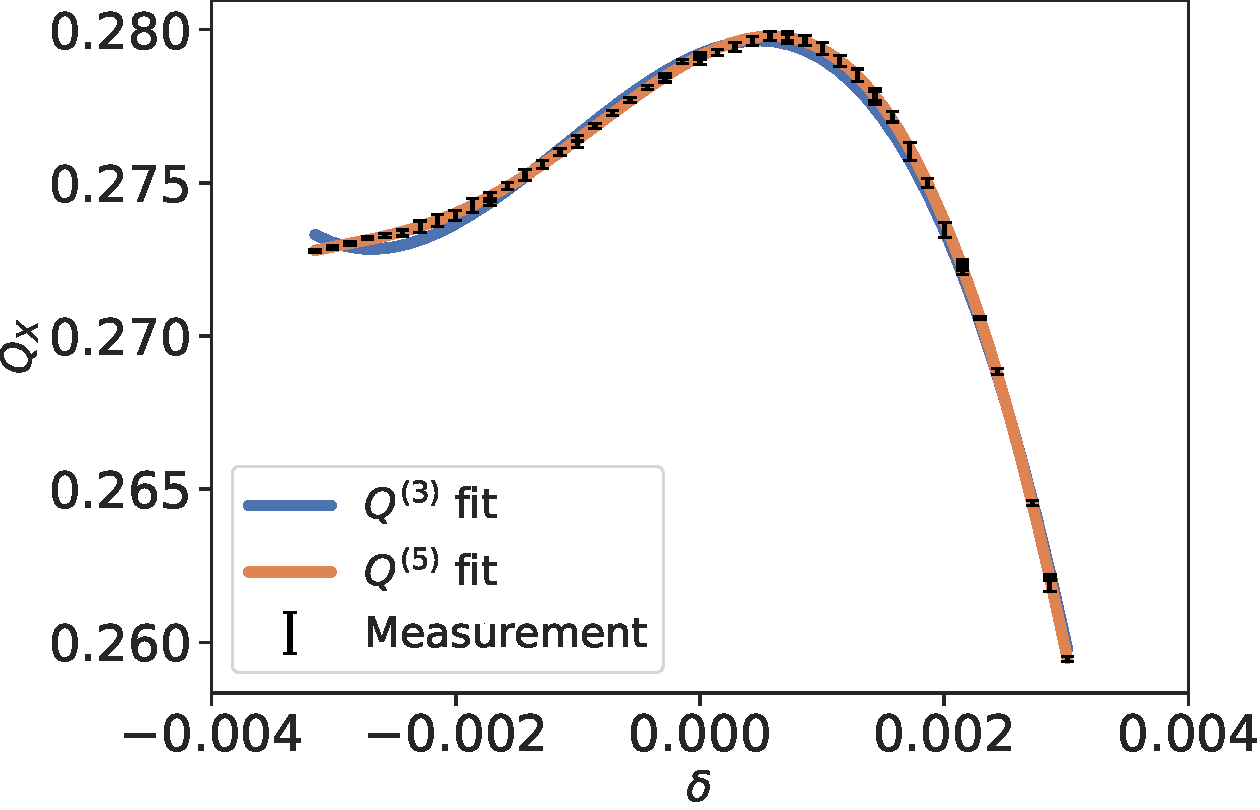
\includegraphics[width=1\columnwidth]{images/MOPL027_f2-1.pdf}
    \caption{Beam 1 measurement of higher order chromaticity terms with nominal corrections used during operation. Fits are up to the third and fifth order.}
    \label[type]{chroma_before_correction}
\end{figure}


%----------------------------------------
%       Beam-Based Corrections
\subsubsection{Beam-Based Corrections}

After correcting the second and third order chromaticities via the octupole and decapole correctors, a
second measurement was performed.
A uniform trim on all the correctors of each class was applied for each beam, resulting in a global correction. A total of four circuits were unavailable for the octupoles, three for beam 1 and one for beam 2, resulting in larger corrections for beam 1.
Corrections applied on top of the nominal settings~\cite{maclean_commissioning_2016} for the octupoles and decapoles are shown in Tab. \ref{mcdo_values_corr}.

\begin{table}[tbh]
    \centering
    \begin{tabular}{|l||r|r|}
    \hline
      Beam  &    $K_4 [\mathrm{m}^{-4}]$      &  $K_5 [\mathrm{m}^{-5}]$  \\ \hline\hline
        1   &  +3.2973     &  +1610   \\ \hline
        2   &   +2.1716    &  +1618   \\ \hline
    \end{tabular}
    \caption{Corrections applied on top of the nominal octupole and decapole correctors strengths.}
    \label{mcdo_values_corr}
\end{table}

Figure \ref{chroma_after_correction} shows the chromaticity fit after the beam-based minimization of $Q''$ and $Q'''$,
while \cref{chroma_table_after} shows the measured chromaticity.

Previous studies of chromaticity in the LHC only considered fits up to third-order.
Including fits up to a fifth order increases the $Q'''$ estimate of both measurements, while improving the fit quality. $Q'''$ for beam 1 with only a fit to the third order would have a value of $-0.38 \times 10^6$
instead of the $-1.02 \times 10^6$ obtained with a fifth order fit. 
Accurately measuring the third order chromaticity is essential in order to correct it.

\begin{figure}[tbh]
    \centering
    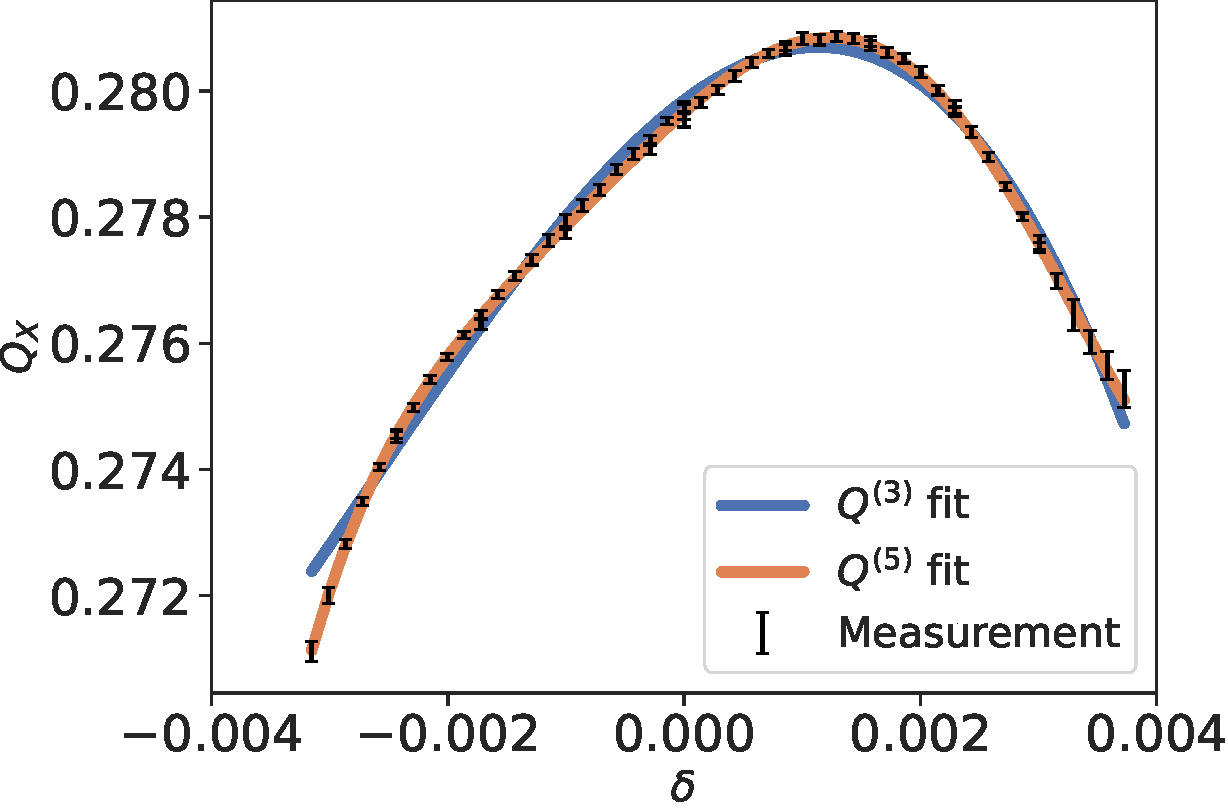
\includegraphics[width=1\columnwidth]{images/MOPL027_f3-1.pdf}
    \caption{Beam 1 measurement of high order chromaticity terms after application of $Q''$ and $Q'''$ 
             beam-based corrections on octupole and decapole correctors.}
    \label{chroma_after_correction}
\end{figure}

\begin{table}[tbh]
    \centering
    \small
    \setlength{\tabcolsep}{4.2pt}
    \begin{tabular}{|l||r|r|r|r|}
    \hline
                 & $Q^{(2)} [10^3]$ & $Q^{(3)} [10^6]$ & $Q^{(4)} [10^9]$ & $Q^{(5)} [10^{12}]$ \\ \hline\hline
        B1    &           &          &              &              \\
        X         & -0.62 ± 0.01     & -1.02 ± 0.03 & -0.63 ± 0.02 &  1.22 ± 0.05 \\
        Y         & -0.24 ± 0.01     & 0.12 ± 0.02 &  0.04 ± 0.02 & -0.56 ± 0.04 \\ \hline
        B2    &           &          &              &              \\
        X         & -0.85 ± 0.01     & -0.64 ± 0.03 & -0.58 ± 0.02 &  1.07 ± 0.06 \\
        Y         & -0.30 ± 0.02     & 0.14 ± 0.03 &  0.16 ± 0.02 & -0.66 ± 0.05 \\ \hline
    \end{tabular}
    \caption{Terms of higher order chromaticity obtained during Run~3 commissioning in April 2022, with beam-based corrections for $Q''$ and $Q'''$.}
    \label{chroma_table_after}
\end{table}


%----------------------------------------
%     Q4 and Q5 confirmation
%----------------------------------------
\subsubsection{\texorpdfstring{$Q^{(4)}$ and $Q^{(5)}$}{Q4 and Q5} fit quality}
\label{subsection:q4q5_quality}

The values measured for $Q^{(4)}$ and $Q^{(5)}$ are similar across the two measurements, with nominal and beam-based corrections performed with very different lower order chromaticity and several hours apart.
This reproducibility gives confidence that the measured values are robust.
It is to be noted that one exception exists, for the horizontal plane of beam 2, where the measurement with nominal correction settings showed a high correlation between the fourth and fifth order terms, making the fit less reliable.

The reduced chi-square for the last measurement for each fit order is detailed in Tab.~\ref{table_chisquare}, where it can be seen that a fit above fifth order does not improve the fit quality.
%Figure \ref{chroma_comparison} shows a comparison of the measured chromaticity before and after
%beam-based corrections for the horizontal axis of beam 1.

\begin{table}[tbh]
    \centering
    \begin{tabular}{|l||c|c|c|c|}
    \hline
        Plane     &  $\chi^2_\nu$ $Q^{(3)}$ & $\chi^2_\nu$ $Q^{(4)}$ &  $\chi^2_\nu$ $Q^{(5)}$ &  $\chi^2_\nu$ $Q^{(6)}$  \\ \hline\hline
        Beam 1    &   &   &   & \\
        % The commented out lines are from measurement with the regular BBQ data
        % The un-commented lines are from using the raw BBQ data
        %X         & 7.62  & 4.07 & 0.62 &\\             % regular
        %Y         & 0.72  & 0.57 & 0.15 &\\ \hline      % regular
        X         & 17.9  & 12.1 & 1.8 & 1.47 \\               % raw bbq
        Y         &  3.0  & 2.2  & 0.7 & 0.7 \\ \hline        % raw bbq
        Beam 2    &    &    &   &\\
        %X         & 7.60  & 3.10 & 0.73 &\\             % regular
        %Y         & 0.48  & 0.46 & 0.16 &\\ \hline      % regular
        X         & 17.3 & 7.1 & 1.8 & 1.76 \\             % raw bbq
        Y         & 2.9  & 2.8 & 1.0 & 1.0 \\ \hline      % raw bbq
    \end{tabular}
    \caption{Reduced $\chi^2_\nu$ values for each order of fit, taken from the last commissioning measurement.}
    \label{table_chisquare}
\end{table}


%\begin{figure}[!ht]
%    \centering
%    \includegraphics[width=1\columnwidth]{images/comparison_b1x.png}
%    \caption{Comparison of the chromaticity function with nominal and beam-based corrections.}
%    \label[type]{chroma_comparison}
%\end{figure}


%----------------------------------------------------------------------------------------
%	    MODEL EXPECTATIONS
%----------------------------------------------------------------------------------------

\subsection{NL-CHROMATICITY MODEL}
\label{sec:nl_chroma_model}

The model of the LHC is based on MADX and WISE field errors~\cite{p_hagen_wise_2006}. To compute the
chromaticity, simulations are run via the Polymorphic Tracking Code (PTC), with field errors from
sextupole to decahexapole loaded and applied on all magnets. Simulation results are shown in Tab.~\ref{ptc_values}.

Table \ref{ptc_values_ratios} shows the ratio between measured and simulated high-order chromaticity. The measured $Q^{(5)}$ shows a consistent discrepancy with the model, larger by about a factor 2.

\begin{table}[tbh]
    \centering
    \small
    \begin{tabular}{|l||r|r|}
    \hline
        Plane     &  $Q^{(4)} [10^9]$  &  $Q^{(5)} 
        [10^{12}]$ \\\hline\hline
        Beam 1    &              &               \\
        X         & -0.2 ± 0.1 & 0.7 ± 0.1  \\
        Y         &  0.1 ± 0.1 & -0.3 ± 0.1  \\ \hline
        Beam 2    &  &   \\
        X         & -0.2 ± 0.1 &  0.8 ± 0.1  \\
        Y         &  0.1 ± 0.1 & -0.4 ± 0.1 \\ \hline
    \end{tabular}
    \caption{Simulated high order chromaticity terms via PTC, including field errors from $b_3$ to $b_8$ with the previous beam-based corrections.}
    \label{ptc_values}
\end{table}

%\begin{table}[tbh]
%    \centering
%    \footnotesize
%    \begin{tabular}{|l||c|c|c|c|}
%    \hline
%        Plane     &  \multicolumn{2}{c|}{$Q^{(4)}$ ratio}   &  \multicolumn{2}{c|}{$Q^{(5)}$ ratio} \\
%        \cline{2-5}
%        Measurement &   first    &    second   &    first   &    second\\ \hline\hline
%        Beam 1    &              &             &            & \\
%        X         &  3.2 ± 0.3   & 3.6 ± 0.3  & 1.8 ± 0.1  & 1.8 ± 0.1  \\
%        Y         &  7.9 ± 2.0   & 2.1 ± 1.1   & 2.7 ± 0.3  & 1.7 ± 0.1  \\ \hline
%        Beam 2    &              &             &            & \\ 
%        X         &              & 4.3 ± 0.4   &            & 1.6 ± 0.1  \\
%        Y         &  18 ± 5      & 12 ± 3      & 2.2 ± 0.4  & 1.9 ± 0.2 \\ \hline
%    \end{tabular}
%    \caption{Ratios of the simulated and measured high order chromaticity terms for both first and second measurements.  The values are taken from tables \ref{chroma_fidel}, \ref{chroma_table_after} and \ref{ptc_values}. The fit with high correlation was not included.}
%    \label{ptc_values_ratios}
%\end{table}
\begin{table}[tbh]
    \centering
    \begin{tabular}{|l||c|c|}
    \hline
        Plane     &  \multicolumn{2}{c|}{$Q^{(5)}$ ratio} \\
        \cline{2-3}
        Measurement &    first   &    second\\ \hline\hline
        Beam 1    &            & \\
        X         &1.8 ± 0.1  & 1.8 ± 0.1  \\
        Y         & 2.7 ± 0.3  & 1.7 ± 0.1  \\ \hline
        Beam 2    &            & \\ 
        X         &            & 1.6 ± 0.1  \\
        Y         & 2.2 ± 0.4  & 1.9 ± 0.2 \\ \hline
    \end{tabular}
    \caption{Ratios of the measured to simulated fifth order chromaticity term for both first and second measurements.  The values are taken from tables~\ref{chroma_fidel}, \ref{chroma_table_after} and \ref{ptc_values}. The fit with high correlation was not included.}
    \label{ptc_values_ratios}
\end{table}


Simulations with only $b_6$ and $b_7$ field errors have been run to assess the contribution of lower order magnets to the fifth order chromaticities. The results strongly imply that the decatetrapole errors are the main contributors to $Q^{(5)}$, as can be seen in Fig.~\ref{beam1_q5x_ptc}.
Fringe fields and skew multipoles have been found to have a negligible impact.
Ongoing studies are assessing the contribution of $\beta$-beating, linear coupling and alignment errors to those estimates.

\begin{figure}[tbh]
    \centering
    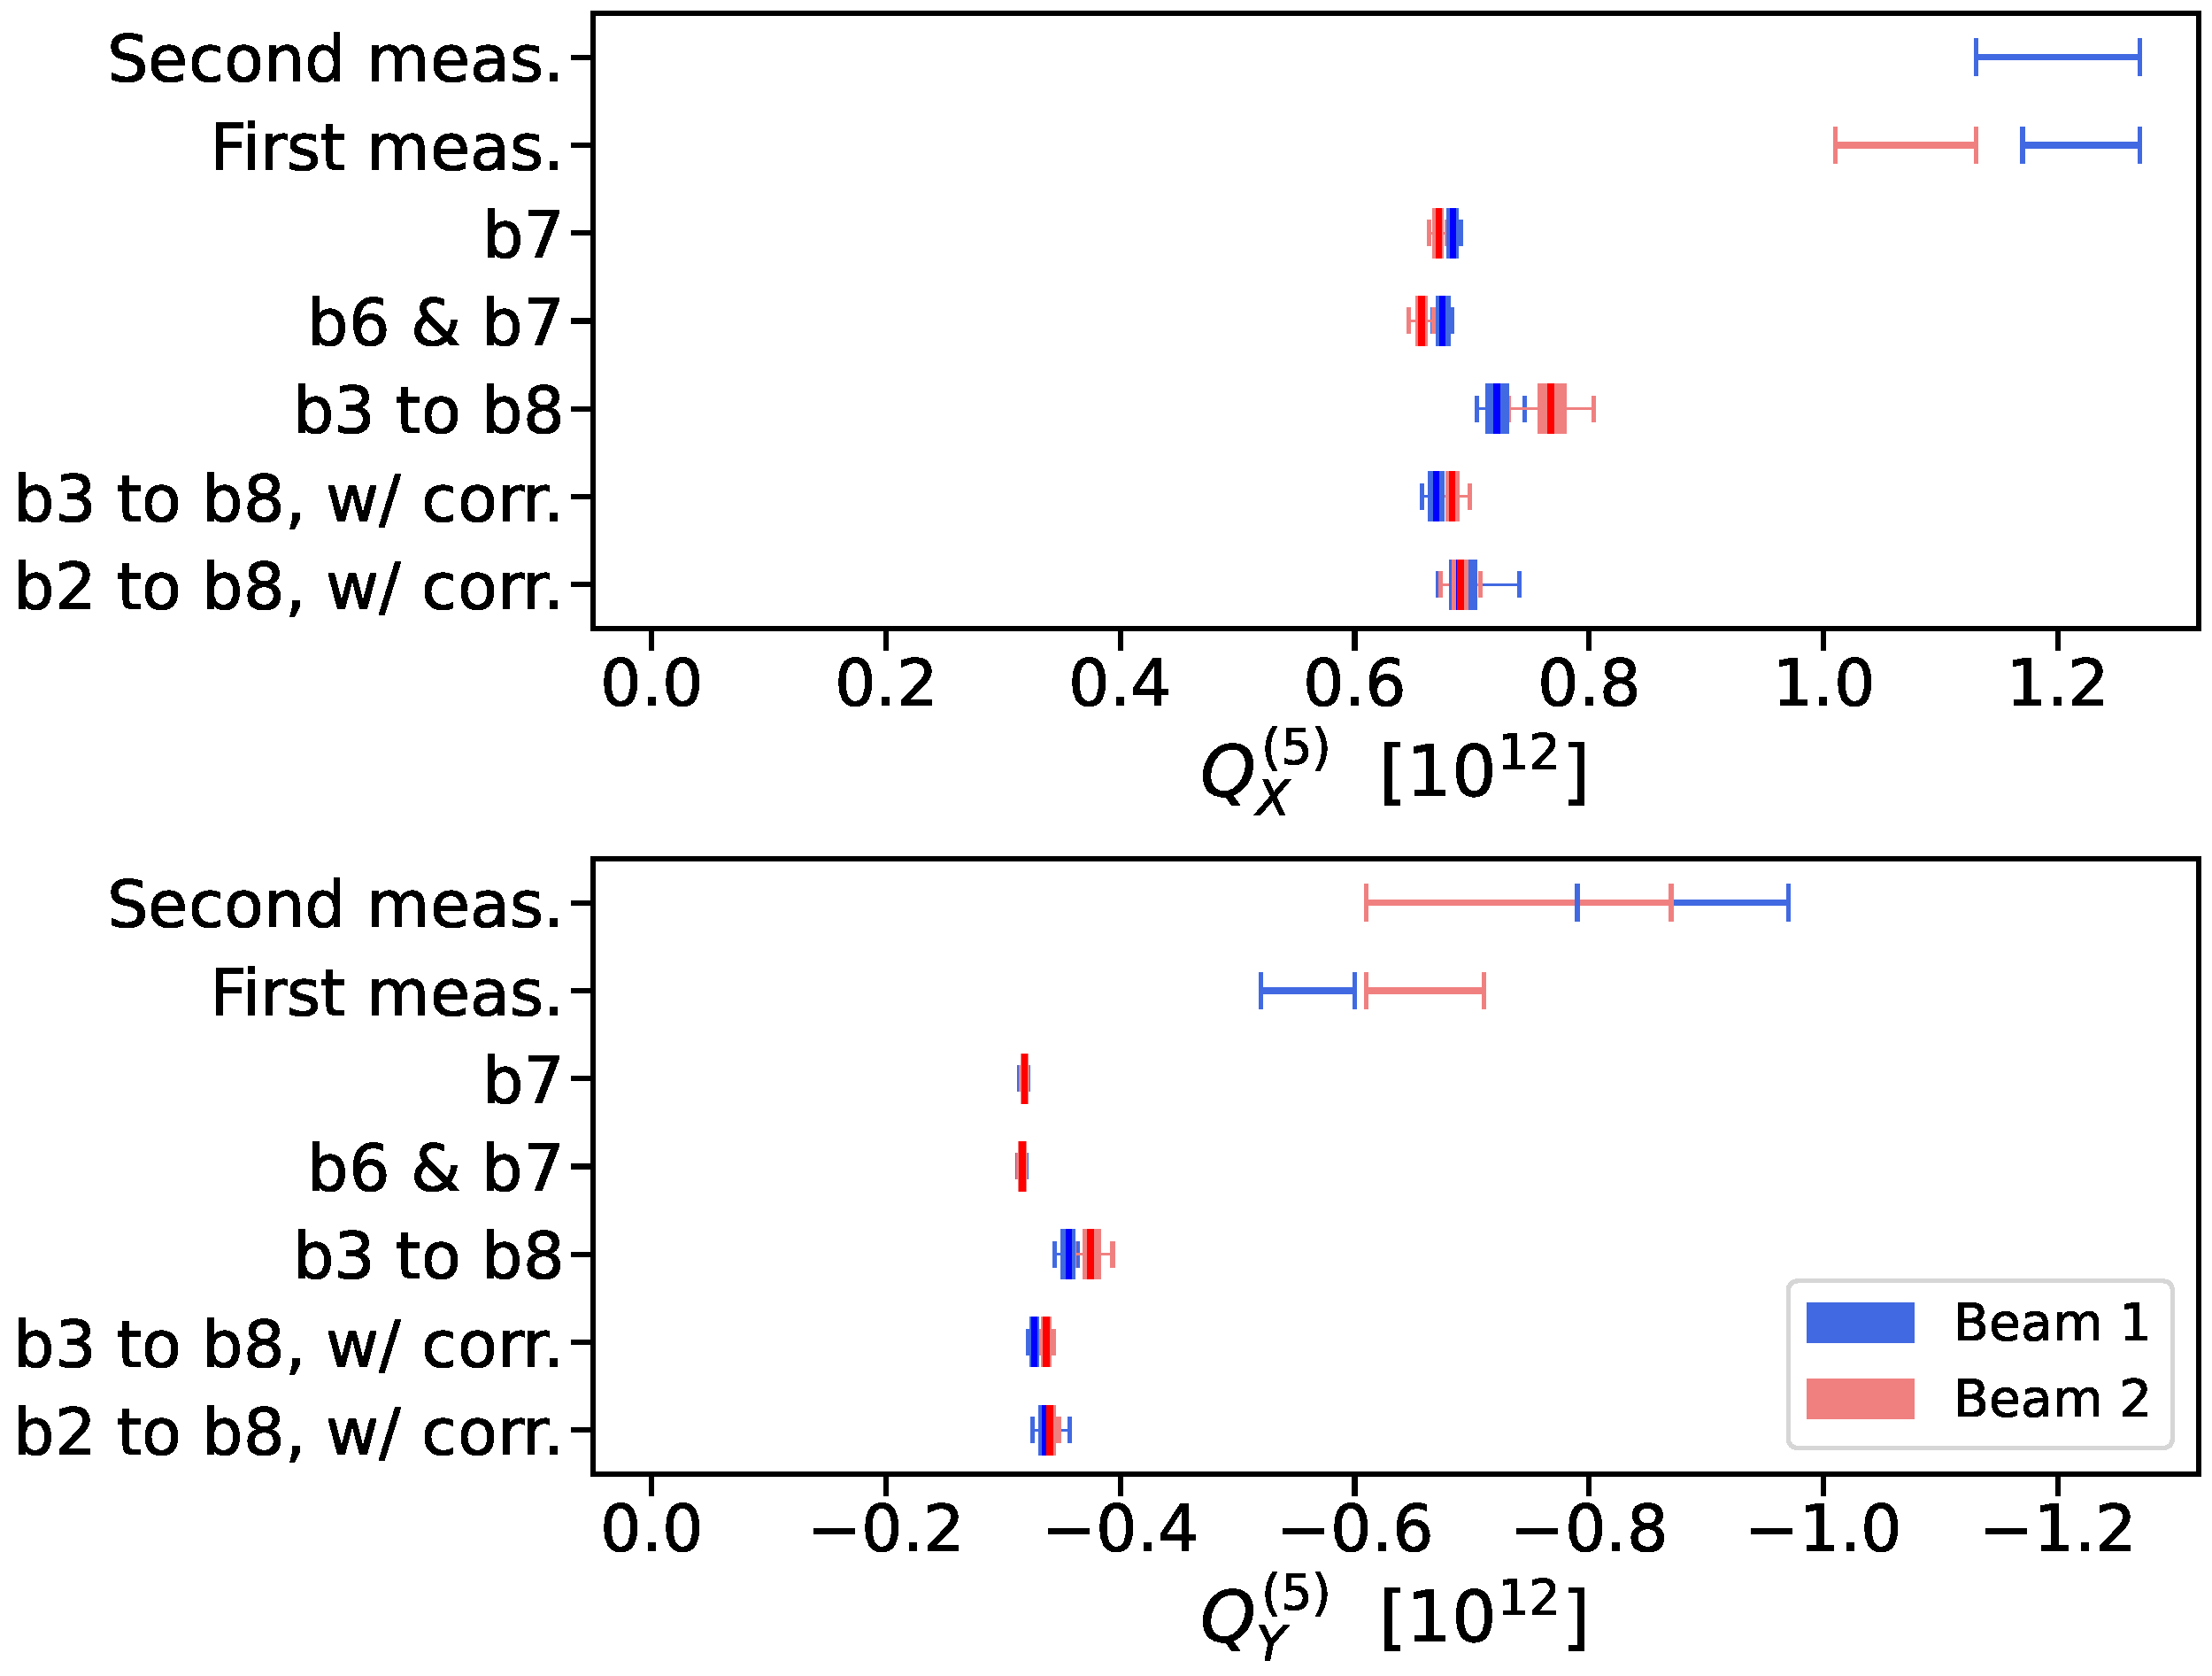
\includegraphics[width=1\columnwidth]{images/MOPL027_f4-1.pdf}
    \caption{Measured and simulated fifth order chromaticity. 
             The simulations are done via PTC and include different multipole errors, some of them further
             include the nominal corrections for $b_3$, $b_4$ and $b_5$.
             The $b_2$ errors, applied on dipoles and quadrupoles, generate beta-beating.
             The measurement with a high correlation is not included.}
    \label{beam1_q5x_ptc}
\end{figure}




%=============================
%            RDTs
%=============================
\section{\todo{First Measurement of Dodecapole RDTs}}

b6 meas from 2024 commissioning




%=============================
%        Conclusion
%=============================
\section{CONCLUSIONS AND OUTLOOK}

A wider momentum offset range, combined with new analysis techniques permitted the observation of fourth and fifth order chromaticity for the first time in the LHC. Reproducible values were measured with different machine configurations.
Preliminary simulations show that the observed values do not match well with the LHC non-linear model. A factor 2 is observed between beams and planes for $Q^{(5)}$, which may point to a systematic error in the b7 error model.

Correction of the measured higher order chromaticity terms is not possible, due to the lack of adequate
correctors in the LHC. It is nevertheless interesting to characterize the higher order errors for an effective model and understand the effect a higher order fit has on lower order terms.
Precise measurement of those lower chromaticity terms is required in order to effectively correct them. 
Higher order terms have thus to be taken into account.

The current range of momentum offset is deemed sufficient to measure higher order chromaticity. Attempts will, however,
be taken to increase that range and assess if such a wider range can refine the estimate of $Q^{(4)}$ and
$Q^{(5)}$.